\section{TidalCycles: Continuous and Discrete Patterns of Functional
Reactive
Programming}\label{tidalcycles-continuous-and-discrete-patterns-of-functional-reactive-programming}

Functional Reactive Programming (FRP) was first introduced by Conal
Elliot as Fran {[}Functional Reactive Animation; @cite{]}, centering on
a definition of behaviour as a continuous function of time. Popular
implementations of FRP, such as in the Elm language, have followed which
have instead opted for discrete rather than continuous semantics. The
following introduces an approach that supports both discrete and
continuous time, that has been developed and popularised over the past
ten years in the TidalCycles system, designed for creative, live
exploration of musical and other patterns.

\subsection{Representing patterns}\label{representing-patterns}

In the following we willi step through the process of building a
representation for musical pattern, taking Elliot's definition of
behaviour in Fran as a worthy starting point. This is done in a
practical, literate programming style, using the Haskell programming
language. We will end up with a that is representation slightly
simplified to but conceptually the same as that used in the TidalCycles
programming language.

Our starting point is the following \texttt{Behaviour} type, based on
Fran's behaviour type:

\begin{Shaded}
\begin{Highlighting}[]
\KeywordTok{type} \DataTypeTok{Time} \OtherTok{=} \DataTypeTok{Double}
\KeywordTok{type} \DataTypeTok{Behaviour}\NormalTok{ a }\OtherTok{=} \DataTypeTok{Time} \OtherTok{{-}\textgreater{}}\NormalTok{ [a]}
\end{Highlighting}
\end{Shaded}

This principled start represents behaviours as functions of time, or in
other words, time-varying values. There might be more than one value
active at a particular point in time, hence the function returns a list
of values.

\subsubsection{Rational time}\label{rational-time}

According to Elliot, \texttt{Time} in FRP should be considered as
\emph{real}, therefore having arbitrary time precision, without building
a notion of samplerate into the representation itself. In practice
though, Fran uses double precision, floating-point numbers for
representing time. Floating point numbers are certainly efficient, but
leave us with the problem of how to deal with floating point errors in
time calculations.

To avoid floating point headaches, here we instead use rational time as
a practical alternative. This fulfills a need that is very common in
computational media: to accurately represent ratios, e.g.~durations of
1/3 for triplets in music, and 1/24 for frame frequencies in video
animation.

\begin{Shaded}
\begin{Highlighting}[]
\KeywordTok{type} \DataTypeTok{Time} \OtherTok{=} \DataTypeTok{Rational}
\KeywordTok{type} \DataTypeTok{Pattern}\NormalTok{ a }\OtherTok{=} \DataTypeTok{Time} \OtherTok{{-}\textgreater{}}\NormalTok{ [a]}
\end{Highlighting}
\end{Shaded}

But this raises a question -- what are these numbers a ratio \emph{of}?
The answer is metric cycles, which in music have particular meaning
depending on your musical tradition. For example in Western music,
metric cycles are referred to as measures or bars, and in Indian music
the more nuanced Tala cycles. Taking inspiration from the latter, in
(the eponymous) TidalCycles they are simply referred as cycles. The
integer timeline (i.e., the ratios with denominator of \texttt{1}) marks
out the endings and beginnings of successive cycles.

We have also renamed our type to \texttt{Pattern} rather than
\texttt{Behaviour}. This both differentiates our type from Elliot's, and
supports our later discussion of relating this representation with the
long history of pattern-making.

\subsubsection{Timespans and events}\label{timespans-and-events}

Next, in order to support discrete events, we introduce the concept of
events with time\emph{spans} to our model. In the following, a timespan
represents the time during which a given event is active.

\begin{Shaded}
\begin{Highlighting}[]
\KeywordTok{data} \DataTypeTok{TimeSpan} \OtherTok{=} \DataTypeTok{TimeSpan}\NormalTok{ \{}\OtherTok{begin ::} \DataTypeTok{Time}\NormalTok{,}\OtherTok{ end ::} \DataTypeTok{Time}\NormalTok{\}}
\KeywordTok{data} \DataTypeTok{Event}\NormalTok{ a }\OtherTok{=} \DataTypeTok{Event}\NormalTok{ \{}\OtherTok{active ::} \DataTypeTok{TimeSpan}\NormalTok{,}\OtherTok{ value ::}\NormalTok{ a\}}
\end{Highlighting}
\end{Shaded}

To support this, we also change our \texttt{Pattern} type to be a
function of time spans, rather than single time values. This is so we
can query the pattern with contiguous time spans, thereby avoiding any
chance of missing events that might otherwise fall between queries.

\begin{Shaded}
\begin{Highlighting}[]
\KeywordTok{type} \DataTypeTok{Pattern}\NormalTok{ a }\OtherTok{=} \DataTypeTok{TimeSpan} \OtherTok{{-}\textgreater{}}\NormalTok{ [}\DataTypeTok{Event}\NormalTok{ a]}
\end{Highlighting}
\end{Shaded}

However, we also need to take into account that an event might well not
fit within the timespan of a given query. We often need to know what
part of an event is active within a timespan, particularly whether it
started before and/or continues beyond that timespan. For this reason,
we add another field to our Event datatype called \texttt{whole},
representing the whole timespan of the event, which might be greater
than the \texttt{active} part, but should always include it.

\begin{Shaded}
\begin{Highlighting}[]
\KeywordTok{data} \DataTypeTok{Event}\NormalTok{ a }\OtherTok{=} \DataTypeTok{Event}\NormalTok{ \{}\OtherTok{whole ::} \DataTypeTok{TimeSpan}\NormalTok{,}\OtherTok{ active ::} \DataTypeTok{TimeSpan}\NormalTok{,}\OtherTok{ value ::}\NormalTok{ a\}}
\end{Highlighting}
\end{Shaded}

Now we turned the \texttt{Pattern} type into one that can represent
discrete events, but it would be best if it could still represent
continuous values. Here, the difference between a discrete and
continuous value is that the latter is never part of a `whole' event.
So, we just need to make that optional.

\begin{Shaded}
\begin{Highlighting}[]
\KeywordTok{data} \DataTypeTok{Event}\NormalTok{ a }\OtherTok{=} \DataTypeTok{Event}\NormalTok{ \{}\OtherTok{whole ::} \DataTypeTok{Maybe} \DataTypeTok{TimeSpan}\NormalTok{,}\OtherTok{ active ::} \DataTypeTok{TimeSpan}\NormalTok{,}\OtherTok{ value ::}\NormalTok{ a\}}
\end{Highlighting}
\end{Shaded}

We can now tell when an event is continuous, because its \texttt{whole}
is set to \texttt{Nothing}.

\subsection{Complete pattern
representation}\label{complete-pattern-representation}

Our representation is now complete, with the following a basis for
representing values that support both continuous and discrete time,
within the same datatype.

\begin{Shaded}
\begin{Highlighting}[]
\KeywordTok{type} \DataTypeTok{Time} \OtherTok{=} \DataTypeTok{Rational}
\KeywordTok{data} \DataTypeTok{TimeSpan} \OtherTok{=} \DataTypeTok{TimeSpan}\NormalTok{ \{}\OtherTok{begin ::} \DataTypeTok{Time}\NormalTok{,}\OtherTok{ end ::} \DataTypeTok{Time}\NormalTok{\}}
    \KeywordTok{deriving} \DataTypeTok{Show}
\KeywordTok{data} \DataTypeTok{Event}\NormalTok{ a }\OtherTok{=} \DataTypeTok{Event}\NormalTok{ \{}\OtherTok{whole ::} \DataTypeTok{Maybe} \DataTypeTok{TimeSpan}\NormalTok{,}\OtherTok{ active ::} \DataTypeTok{TimeSpan}\NormalTok{,}\OtherTok{ value ::}\NormalTok{ a\}}
    \KeywordTok{deriving}\NormalTok{ (}\DataTypeTok{Show}\NormalTok{, }\DataTypeTok{Functor}\NormalTok{)}
\KeywordTok{data} \DataTypeTok{Pattern}\NormalTok{ a }\OtherTok{=} \DataTypeTok{Pattern}\NormalTok{ \{}\OtherTok{query ::} \DataTypeTok{TimeSpan} \OtherTok{{-}\textgreater{}}\NormalTok{ [}\DataTypeTok{Event}\NormalTok{ a]\}}
    \KeywordTok{deriving}\NormalTok{ (}\DataTypeTok{Functor}\NormalTok{)}
\end{Highlighting}
\end{Shaded}

\subsection{Constructing patterns}\label{constructing-patterns}

How does this work in practice? For continuous patterns, we simply
sample a value at the halfway point of the given timespan. For example,
a sinewave:

\begin{Shaded}
\begin{Highlighting}[]
\OtherTok{sinewave ::} \DataTypeTok{Pattern} \DataTypeTok{Double}
\NormalTok{sinewave }\OtherTok{=} \DataTypeTok{Pattern} \OperatorTok{$}\NormalTok{ \textbackslash{}timespan }\OtherTok{{-}\textgreater{}}\NormalTok{ [}\DataTypeTok{Event} \DataTypeTok{Nothing}\NormalTok{ timespan }\OperatorTok{$} \FunctionTok{sin} \OperatorTok{$}\NormalTok{ (}\FunctionTok{fromRational} \OperatorTok{$}\NormalTok{ t timespan) }\OperatorTok{*} \FunctionTok{pi} \OperatorTok{*} \DecValTok{2}\NormalTok{]}
    \KeywordTok{where}\NormalTok{ t timespan }\OtherTok{=}\NormalTok{ begin timespan }\OperatorTok{+}\NormalTok{ ((end timespan }\OperatorTok{{-}}\NormalTok{ begin timespan) }\OperatorTok{/} \DecValTok{2}\NormalTok{)}
\end{Highlighting}
\end{Shaded}

For discrete patterns, we need to supply both the whole and part. For
example, to repeat a discrete value with a duration of one `cycle', we
can use the \texttt{atom} function:

\begin{Shaded}
\begin{Highlighting}[]
\NormalTok{sam,}\OtherTok{ nextSam ::} \DataTypeTok{Rational} \OtherTok{{-}\textgreater{}} \DataTypeTok{Rational}
\NormalTok{sam t }\OtherTok{=} \FunctionTok{toRational}\NormalTok{ (}\FunctionTok{floor}\OtherTok{ t ::} \DataTypeTok{Int}\NormalTok{)}
\NormalTok{nextSam }\OtherTok{=}\NormalTok{ (}\DecValTok{1} \OperatorTok{+}\NormalTok{) }\OperatorTok{.}\NormalTok{ sam}

\OtherTok{splitSpan ::} \DataTypeTok{TimeSpan} \OtherTok{{-}\textgreater{}}\NormalTok{ [}\DataTypeTok{TimeSpan}\NormalTok{]}
\NormalTok{splitSpan (}\DataTypeTok{TimeSpan}\NormalTok{ s e) }\OperatorTok{|}\NormalTok{ sam s }\OperatorTok{==}\NormalTok{ sam e }\OperatorTok{||}\NormalTok{ n }\OperatorTok{==}\NormalTok{ e }\OtherTok{=}\NormalTok{ [}\DataTypeTok{TimeSpan}\NormalTok{ s e]}
                         \OperatorTok{|} \FunctionTok{otherwise} \OtherTok{=} \DataTypeTok{TimeSpan}\NormalTok{ s n }\OperatorTok{:}\NormalTok{ splitSpan (}\DataTypeTok{TimeSpan}\NormalTok{ n e)}
    \KeywordTok{where}\NormalTok{ n }\OtherTok{=}\NormalTok{ nextSam s}

\OtherTok{atom ::}\NormalTok{ a }\OtherTok{{-}\textgreater{}} \DataTypeTok{Pattern}\NormalTok{ a}
\NormalTok{atom v }\OtherTok{=} \DataTypeTok{Pattern} \OperatorTok{$} \FunctionTok{map}\NormalTok{ (\textbackslash{}timespan }\OtherTok{{-}\textgreater{}} \DataTypeTok{Event}\NormalTok{ (}\DataTypeTok{Just} \OperatorTok{$} \DataTypeTok{TimeSpan}\NormalTok{ (sam }\OperatorTok{$}\NormalTok{ begin timespan) (nextSam }\OperatorTok{$}\NormalTok{ begin timespan)) timespan v) }\OperatorTok{.}\NormalTok{ splitSpan}
\end{Highlighting}
\end{Shaded}

\subsection{Manipulating time}\label{manipulating-time}

One good thing about pure FRP is that it is possible to manipulate time,
simply by making a new pattern function that calls the old one,
adjusting time values passed to its query on the way. Because the above
representation has timespans in two places -- in the query and the
events that result -- we must be careful to adjust both. We therefore
require two functions for every time manipulation, one to adjust the
query, and another to adjust the result, so that the timespans of events
are still active within the queried timespan. To make that easy, here
are some utility functions for working with query and event time:

\begin{Shaded}
\begin{Highlighting}[]
\OtherTok{withSpanTime ::}\NormalTok{ (}\DataTypeTok{Time} \OtherTok{{-}\textgreater{}} \DataTypeTok{Time}\NormalTok{) }\OtherTok{{-}\textgreater{}} \DataTypeTok{TimeSpan} \OtherTok{{-}\textgreater{}} \DataTypeTok{TimeSpan}
\NormalTok{withSpanTime timef (}\DataTypeTok{TimeSpan}\NormalTok{ b e) }\OtherTok{=} \DataTypeTok{TimeSpan}\NormalTok{ (timef b) (timef e)}

\OtherTok{withQueryTime ::}\NormalTok{ (}\DataTypeTok{Time} \OtherTok{{-}\textgreater{}} \DataTypeTok{Time}\NormalTok{) }\OtherTok{{-}\textgreater{}} \DataTypeTok{Pattern}\NormalTok{ a }\OtherTok{{-}\textgreater{}} \DataTypeTok{Pattern}\NormalTok{ a}
\NormalTok{withQueryTime timef (}\DataTypeTok{Pattern}\NormalTok{ q) }\OtherTok{=} \DataTypeTok{Pattern} \OperatorTok{$}\NormalTok{ q }\OperatorTok{.}\NormalTok{ withSpanTime timef}

\OtherTok{withEventTime ::}\NormalTok{ (}\DataTypeTok{Time} \OtherTok{{-}\textgreater{}} \DataTypeTok{Time}\NormalTok{) }\OtherTok{{-}\textgreater{}} \DataTypeTok{Pattern}\NormalTok{ a }\OtherTok{{-}\textgreater{}} \DataTypeTok{Pattern}\NormalTok{ a}
\NormalTok{withEventTime f }\OtherTok{=}\NormalTok{ withEvent }\OperatorTok{$}\NormalTok{ \textbackslash{}e }\OtherTok{{-}\textgreater{}}\NormalTok{ e \{active }\OtherTok{=}\NormalTok{ withSpanTime f }\OperatorTok{$}\NormalTok{ active e,}
\NormalTok{                                       whole }\OtherTok{=}\NormalTok{ withSpanTime f }\OperatorTok{\textless{}$\textgreater{}}\NormalTok{ whole e}
\NormalTok{                                      \}}
    \KeywordTok{where}\NormalTok{ withEvent ef (}\DataTypeTok{Pattern}\NormalTok{ q) }\OtherTok{=} \DataTypeTok{Pattern} \OperatorTok{$} \FunctionTok{map}\NormalTok{ ef }\OperatorTok{\textless{}$\textgreater{}}\NormalTok{ q}

\OtherTok{withTime ::}\NormalTok{ (}\DataTypeTok{Time} \OtherTok{{-}\textgreater{}} \DataTypeTok{Time}\NormalTok{) }\OtherTok{{-}\textgreater{}}\NormalTok{ (}\DataTypeTok{Time} \OtherTok{{-}\textgreater{}} \DataTypeTok{Time}\NormalTok{) }\OtherTok{{-}\textgreater{}} \DataTypeTok{Pattern}\NormalTok{ a }\OtherTok{{-}\textgreater{}} \DataTypeTok{Pattern}\NormalTok{ a}
\NormalTok{withTime fa fb pat }\OtherTok{=}\NormalTok{ withEventTime fa }\OperatorTok{$}\NormalTok{ withQueryTime fb pat}
\end{Highlighting}
\end{Shaded}

We can now make functions for making events faster/slower, or
early/late.

\begin{Shaded}
\begin{Highlighting}[]
\NormalTok{\_fast, \_slow, \_late,}\OtherTok{ \_early ::} \DataTypeTok{Time} \OtherTok{{-}\textgreater{}} \DataTypeTok{Pattern}\NormalTok{ a }\OtherTok{{-}\textgreater{}} \DataTypeTok{Pattern}\NormalTok{ a}
\NormalTok{\_fast t  }\OtherTok{=}\NormalTok{ withEventTime (}\OperatorTok{/}\NormalTok{ t) }\OperatorTok{.}\NormalTok{ withQueryTime (}\OperatorTok{*}\NormalTok{ t)}
\NormalTok{\_slow t  }\OtherTok{=}\NormalTok{ withEventTime (}\OperatorTok{*}\NormalTok{ t) }\OperatorTok{.}\NormalTok{ withQueryTime (}\OperatorTok{/}\NormalTok{ t)}
\NormalTok{\_early t }\OtherTok{=}\NormalTok{ withEventTime (}\FunctionTok{subtract}\NormalTok{ t) }\OperatorTok{.}\NormalTok{ withQueryTime (}\OperatorTok{+}\NormalTok{ t)}
\NormalTok{\_late t  }\OtherTok{=}\NormalTok{ withEventTime (}\OperatorTok{+}\NormalTok{ t) }\OperatorTok{.}\NormalTok{ withQueryTime (}\FunctionTok{subtract}\NormalTok{ t)}
\end{Highlighting}
\end{Shaded}

For example in the above, to make a pattern `faster', we both divide
query time by a given factor, and multiply event time by that same given
factor. In so doing we query a wider window for more events, that then
`squash' back into requested timespan.

\subsection{Combining patterns}\label{combining-patterns}

We can most combine a list of patterns concurrently, by simply applying
the same query to them all:

\begin{Shaded}
\begin{Highlighting}[]
\OtherTok{stack ::}\NormalTok{ [}\DataTypeTok{Pattern}\NormalTok{ a] }\OtherTok{{-}\textgreater{}} \DataTypeTok{Pattern}\NormalTok{ a}
\NormalTok{stack pats }\OtherTok{=} \DataTypeTok{Pattern} \OperatorTok{$}\NormalTok{ \textbackslash{}timespan }\OtherTok{{-}\textgreater{}} \FunctionTok{concatMap}\NormalTok{ (}\OtherTok{\textasciigrave{}query\textasciigrave{}}\NormalTok{ timespan) pats}
\end{Highlighting}
\end{Shaded}

Slightly more complicated is combining them over time. Because patterns
have infinite length, we are not able to concatenate them. Instead, we
can `interlace' cycles, which correspond to the integer timeline.

\begin{Shaded}
\begin{Highlighting}[]
\OtherTok{splitQueries ::} \DataTypeTok{Pattern}\NormalTok{ a }\OtherTok{{-}\textgreater{}} \DataTypeTok{Pattern}\NormalTok{ a}
\NormalTok{splitQueries pat }\OtherTok{=}  \DataTypeTok{Pattern} \OperatorTok{$} \FunctionTok{concatMap}\NormalTok{ (query pat) }\OperatorTok{.}\NormalTok{ splitSpan}

\OtherTok{interlace ::}\NormalTok{ [}\DataTypeTok{Pattern}\NormalTok{ a] }\OtherTok{{-}\textgreater{}} \DataTypeTok{Pattern}\NormalTok{ a}
\NormalTok{interlace pats }\OtherTok{=}\NormalTok{ splitQueries }\OperatorTok{$} \DataTypeTok{Pattern}\NormalTok{ f}
  \KeywordTok{where}\NormalTok{ f timespan }\OtherTok{=}\NormalTok{ query (\_late offset pat) timespan}
              \KeywordTok{where}\NormalTok{ n }\OtherTok{=} \FunctionTok{toRational} \OperatorTok{$} \FunctionTok{length}\NormalTok{ pats}
\NormalTok{                    cyc }\OtherTok{=}\NormalTok{ sam }\OperatorTok{$}\NormalTok{ begin timespan}
\NormalTok{                    pat }\OtherTok{=}\NormalTok{ pats }\OperatorTok{!!} \FunctionTok{floor}\NormalTok{ (cyc }\OtherTok{\textasciigrave{}mod\textquotesingle{}\textasciigrave{}}\NormalTok{ (}\OtherTok{n ::} \DataTypeTok{Rational}\NormalTok{))}
\NormalTok{                    offset }\OtherTok{=}\NormalTok{ cyc }\OperatorTok{{-}}\NormalTok{ sam (begin timespan }\OperatorTok{/}\NormalTok{ n)}
\end{Highlighting}
\end{Shaded}

Let's look at a visualisation of the first six cycles of a pattern
composed using both \texttt{interlace} and \texttt{stack}. In the
following time is from left to right, with the vertical axis used to
show simultaneously occuring events.

\begin{Shaded}
\begin{Highlighting}[]
\NormalTok{fig1 }\OtherTok{=}\NormalTok{ stack [atom }\StringTok{"red"}\NormalTok{, interlace [atom }\StringTok{"pink"}\NormalTok{, atom }\StringTok{"purple"}\NormalTok{]]}
\end{Highlighting}
\end{Shaded}

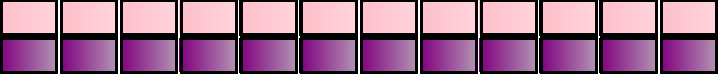
\includegraphics{../figures/fig1.pdf}\\

We can apply this visualisation in understanding how events can become
broken up. If \texttt{interlace} works cycle-by-cycle, what happens if
an event lasts longer than a cycle?

\begin{Shaded}
\begin{Highlighting}[]
\NormalTok{fig2 }\OtherTok{=}\NormalTok{ interlace [atom }\StringTok{"orange"}\NormalTok{, \_slow }\DecValTok{2} \OperatorTok{$}\NormalTok{ atom }\StringTok{"red"}\NormalTok{]}
\end{Highlighting}
\end{Shaded}

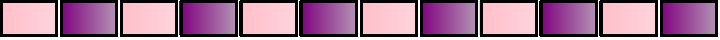
\includegraphics{../figures/fig2.pdf}\\

From the above we can see that the `whole' red events last two cycles,
but each is broken in two `active' parts lasting one cycle each. The red
portion represents the active part, and the lighter red (pink) portion
represents the rest of the `whole'.

\subsection{Combining patterns with monadic
binds}\label{combining-patterns-with-monadic-binds}

On these foundations, we can begin building a domain specific language.
The above functions are prefixed by \texttt{\_}, because they are
considered internal functions and not part of the end-user interface.
The reason for this is that in TidalCycles, \emph{everything} is a
pattern. So we require functions with the following time signature:

\begin{Shaded}
\begin{Highlighting}[]
\NormalTok{fast, slow, late,}\OtherTok{ early ::} \DataTypeTok{Pattern} \DataTypeTok{Time} \OtherTok{{-}\textgreater{}} \DataTypeTok{Pattern}\NormalTok{ a }\OtherTok{{-}\textgreater{}} \DataTypeTok{Pattern}\NormalTok{ a}
\end{Highlighting}
\end{Shaded}

This is where Haskell's monadic bind
(\texttt{\textgreater{}\textgreater{}=}) comes into view, which supports
the lifting of functional arguments into contexts like our patterns. In
other words, defining our Pattern type as an instance of Haskell's
standard Monad typeclass will solve this problem (and many others to
come). However we do need to define the bind operator
\texttt{\textgreater{}\textgreater{}=} for patterns, with the type
signature
\texttt{Pattern\ a\ -\textgreater{}\ (a\ -\textgreater{}\ Pattern\ b)\ -\textgreater{}\ Pattern\ b}.
The question is, what should this bind do?

Certainly, our bind will need to create a new pattern, which as we saw
above, will be a function from timespans to events. This function will
need to be composed of other patterns, in particular the `outer'
function given as the first argument, and `inner' functions resulting
from the second argument. The biggest question here is deciding how to
deal with the timespans of events when composing these patterns
together.

In the bind, the resulting pattern function will pass on its query to
the `outer' pattern function, then for each event returned by it, pass
the event's value to the binding function, then use the event's active
timespan to query the `inner' pattern returned by the binding function.
The events returned by the `inner' pattern should then fall within the
timespan of the outer events.

The events returned from those inner pattern queries are then collated
and returned, with one caveat -- there is ambiguity about what the
resulting event's `whole' timespan should be. It could from from the
`outer' or `inner' pattern, or be the intersection of the two. In
practice, the question is about where pattern \emph{structure} shoul
come from - should we preserve the structure of the outer pattern, the
inner pattern, or a combination of the two? In the case of the above
\texttt{fast} function and it's \texttt{slow}, \texttt{late} and
\texttt{early} friends, we can say that we want to preserve the
structure of the inner patterns - the patterns of values which come
second in the functions' arguments. This is because we only want to
transform a value pattern using a time pattern, but not otherwise change
the value pattern's structure. We will see examples of functions that do
change the structure of events later.

The following shows how inner, outer and `mix' binds can be implemented.

\begin{Shaded}
\begin{Highlighting}[]
\OtherTok{bindWith ::}\NormalTok{ (}\DataTypeTok{Maybe} \DataTypeTok{TimeSpan} \OtherTok{{-}\textgreater{}} \DataTypeTok{Maybe} \DataTypeTok{TimeSpan} \OtherTok{{-}\textgreater{}} \DataTypeTok{Maybe} \DataTypeTok{TimeSpan}\NormalTok{) }\OtherTok{{-}\textgreater{}} \DataTypeTok{Pattern}\NormalTok{ a }\OtherTok{{-}\textgreater{}}\NormalTok{ (a }\OtherTok{{-}\textgreater{}} \DataTypeTok{Pattern}\NormalTok{ b) }\OtherTok{{-}\textgreater{}} \DataTypeTok{Pattern}\NormalTok{ b}
\NormalTok{bindWith chooseWhole bv f }\OtherTok{=} \DataTypeTok{Pattern} \OperatorTok{$} \FunctionTok{concatMap}\NormalTok{ match }\OperatorTok{.}\NormalTok{ query bv}
  \KeywordTok{where}\NormalTok{ match event }\OtherTok{=} \FunctionTok{map}\NormalTok{ (withWhole event) }\OperatorTok{$}\NormalTok{ query (f }\OperatorTok{$}\NormalTok{ value event) }\OperatorTok{$}\NormalTok{ active event}
\NormalTok{        withWhole event event\textquotesingle{} }\OtherTok{=}\NormalTok{ event\textquotesingle{} \{whole }\OtherTok{=}\NormalTok{ chooseWhole (whole event) (whole event\textquotesingle{})\}}

\OtherTok{innerBind ::} \DataTypeTok{Pattern}\NormalTok{ a }\OtherTok{{-}\textgreater{}}\NormalTok{ (a }\OtherTok{{-}\textgreater{}} \DataTypeTok{Pattern}\NormalTok{ b) }\OtherTok{{-}\textgreater{}} \DataTypeTok{Pattern}\NormalTok{ b}
\NormalTok{innerBind }\OtherTok{=}\NormalTok{ bindWith (}\FunctionTok{flip} \FunctionTok{const}\NormalTok{)}

\OtherTok{outerBind ::} \DataTypeTok{Pattern}\NormalTok{ a }\OtherTok{{-}\textgreater{}}\NormalTok{ (a }\OtherTok{{-}\textgreater{}} \DataTypeTok{Pattern}\NormalTok{ b) }\OtherTok{{-}\textgreater{}} \DataTypeTok{Pattern}\NormalTok{ b}
\NormalTok{outerBind }\OtherTok{=}\NormalTok{ bindWith }\FunctionTok{const}

\OtherTok{mixBind ::} \DataTypeTok{Pattern}\NormalTok{ a }\OtherTok{{-}\textgreater{}}\NormalTok{ (a }\OtherTok{{-}\textgreater{}} \DataTypeTok{Pattern}\NormalTok{ b) }\OtherTok{{-}\textgreater{}} \DataTypeTok{Pattern}\NormalTok{ b}
\NormalTok{mixBind }\OtherTok{=}\NormalTok{ bindWith (liftA2 intersect)}
\end{Highlighting}
\end{Shaded}

So by taking the intersection of the event wholes, we are combining the
time structures of the two patterns in what we term a `mix' bind.
Alternatively we could do an `inner' bind by using the time structure of
the inner pattern, or an `outer' bind by using the outer structure. The
default bind in the \texttt{Monad} instance is set as a
\texttt{mixBind}. We also define straightforward \texttt{Monoid} and
\texttt{Applicative} instances.

\begin{Shaded}
\begin{Highlighting}[]
\KeywordTok{instance} \DataTypeTok{Monad} \DataTypeTok{Pattern} \KeywordTok{where}
\NormalTok{  (}\OperatorTok{\textgreater{}\textgreater{}=}\NormalTok{) }\OtherTok{=}\NormalTok{ mixBind}

\KeywordTok{instance} \DataTypeTok{Applicative} \DataTypeTok{Pattern} \KeywordTok{where}
  \FunctionTok{pure} \OtherTok{=}\NormalTok{ atom}
\NormalTok{  pf }\OperatorTok{\textless{}*\textgreater{}}\NormalTok{ px }\OtherTok{=}\NormalTok{ pf }\OperatorTok{\textgreater{}\textgreater{}=}\NormalTok{ (}\OperatorTok{\textless{}$\textgreater{}}\NormalTok{ px)}
\end{Highlighting}
\end{Shaded}

Using this, we can make a function \texttt{patternify\_x} that lifts a
function's first argument into a pattern, using \texttt{innerBind} to
preserve the structure of the second argument. This can then be used to
define our \texttt{fast}, \texttt{slow}, \texttt{late} and
\texttt{early} functions.

\begin{Shaded}
\begin{Highlighting}[]
\OtherTok{patternify\_x ::}\NormalTok{ (a }\OtherTok{{-}\textgreater{}} \DataTypeTok{Pattern}\NormalTok{ b }\OtherTok{{-}\textgreater{}} \DataTypeTok{Pattern}\NormalTok{ c) }\OtherTok{{-}\textgreater{}}\NormalTok{ (}\DataTypeTok{Pattern}\NormalTok{ a }\OtherTok{{-}\textgreater{}} \DataTypeTok{Pattern}\NormalTok{ b }\OtherTok{{-}\textgreater{}} \DataTypeTok{Pattern}\NormalTok{ c)}
\NormalTok{patternify\_x f ba bb }\OtherTok{=}\NormalTok{ ba }\OtherTok{\textasciigrave{}innerBind\textasciigrave{}}\NormalTok{ \textbackslash{}a }\OtherTok{{-}\textgreater{}}\NormalTok{ f a bb}

\NormalTok{fast, slow, late,}\OtherTok{ early ::} \DataTypeTok{Pattern} \DataTypeTok{Time} \OtherTok{{-}\textgreater{}} \DataTypeTok{Pattern}\NormalTok{ a }\OtherTok{{-}\textgreater{}} \DataTypeTok{Pattern}\NormalTok{ a}
\NormalTok{fast }\OtherTok{=}\NormalTok{ patternify\_x \_fast}
\NormalTok{slow }\OtherTok{=}\NormalTok{ patternify\_x \_slow}
\NormalTok{late }\OtherTok{=}\NormalTok{ patternify\_x \_late}
\NormalTok{early }\OtherTok{=}\NormalTok{ patternify\_x \_early}
\end{Highlighting}
\end{Shaded}

\begin{Shaded}
\begin{Highlighting}[]
\NormalTok{fig3 }\OtherTok{=}\NormalTok{ fast (atom }\DecValTok{2}\NormalTok{) }\OperatorTok{$}\NormalTok{ atom }\StringTok{"orange"}
\end{Highlighting}
\end{Shaded}

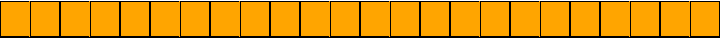
\includegraphics{../figures/fig3.pdf}\\

\begin{Shaded}
\begin{Highlighting}[]
\NormalTok{fig4 }\OtherTok{=}\NormalTok{ slow (atom }\DecValTok{2}\NormalTok{) }\OperatorTok{$}\NormalTok{ atom }\StringTok{"orange"}
\end{Highlighting}
\end{Shaded}

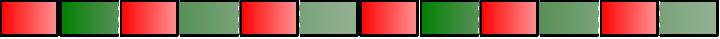
\includegraphics{../figures/fig4.pdf}\\

\subsubsection{Masking and restructuring
patterns}\label{masking-and-restructuring-patterns}

So far we have manipulated time, but not structure.

\begin{Shaded}
\begin{Highlighting}[]
\OtherTok{silence ::} \DataTypeTok{Pattern}\NormalTok{ a}
\NormalTok{silence }\OtherTok{=} \DataTypeTok{Pattern} \OperatorTok{$} \FunctionTok{const}\NormalTok{ []}

\OtherTok{\_ifpat ::} \DataTypeTok{Bool} \OtherTok{{-}\textgreater{}} \DataTypeTok{Pattern}\NormalTok{ a }\OtherTok{{-}\textgreater{}} \DataTypeTok{Pattern}\NormalTok{ a}
\NormalTok{\_ifpat }\DataTypeTok{True}\NormalTok{ p }\OtherTok{=}\NormalTok{ p}
\NormalTok{\_ifpat }\DataTypeTok{False}\NormalTok{ \_ }\OtherTok{=}\NormalTok{ silence}

\OtherTok{mask ::} \DataTypeTok{Pattern} \DataTypeTok{Bool} \OtherTok{{-}\textgreater{}} \DataTypeTok{Pattern}\NormalTok{ a }\OtherTok{{-}\textgreater{}} \DataTypeTok{Pattern}\NormalTok{ a}
\NormalTok{mask bp p }\OtherTok{=}\NormalTok{ bp }\OtherTok{\textasciigrave{}outerBind\textasciigrave{}}\NormalTok{ \textbackslash{}b }\OtherTok{{-}\textgreater{}}\NormalTok{ \_ifpat b p}

\OtherTok{struct ::} \DataTypeTok{Pattern} \DataTypeTok{Bool} \OtherTok{{-}\textgreater{}} \DataTypeTok{Pattern}\NormalTok{ a }\OtherTok{{-}\textgreater{}} \DataTypeTok{Pattern}\NormalTok{ a}
\NormalTok{struct bp p }\OtherTok{=}\NormalTok{ bp }\OtherTok{\textasciigrave{}innerBind\textasciigrave{}}\NormalTok{ \textbackslash{}b }\OtherTok{{-}\textgreater{}}\NormalTok{ \_ifpat b p}
\end{Highlighting}
\end{Shaded}

\appendix

\section{Preamble and supporting
functions}\label{preamble-and-supporting-functions}

\begin{Shaded}
\begin{Highlighting}[]
\KeywordTok{module} \DataTypeTok{Pattern} \KeywordTok{where}

\KeywordTok{import} \DataTypeTok{Control.Applicative}
\KeywordTok{import} \DataTypeTok{Data.Fixed}

\OtherTok{intersect ::} \DataTypeTok{TimeSpan} \OtherTok{{-}\textgreater{}} \DataTypeTok{TimeSpan} \OtherTok{{-}\textgreater{}} \DataTypeTok{TimeSpan}
\NormalTok{intersect (}\DataTypeTok{TimeSpan}\NormalTok{ b e) (}\DataTypeTok{TimeSpan}\NormalTok{ b\textquotesingle{} e\textquotesingle{}) }\OtherTok{=} \DataTypeTok{TimeSpan}\NormalTok{ (}\FunctionTok{max}\NormalTok{ b b\textquotesingle{}) (}\FunctionTok{min}\NormalTok{ e e\textquotesingle{})}
\end{Highlighting}
\end{Shaded}
